Based on a proposed bug taxonomy for Go \cite{tu-concurrentBugs-asplos19}, bugs are categorized separately based on their \textit{causes} (shared-memory vs. message-passing) and \textit{symptoms} (blocking vs. non-blocking).
%
Blocking bugs historically refer to situations where one or more processing units (\eg goroutines) are blocked, waiting for an external signal to resume (\ie deadlocks).
%
As mentioned in section \ref{sec:bg}, the built-in deadlock detector (if not disabled \cite{go-netDeadlock}) only detects global deadlocks where the main goroutine is blocked and ignores other goroutines' states. For instance, more than 70\% of blocking bugs (partial deadlocks and leaks) in GoKer \cite{GoKer} are not detectable by the built-in deadlock detector.
%

As we have shown in our previous work \cite{parlot,difftrace}, dynamic tracing is an effective way in debugging large-scale applications.
%
We found that Go execution tracer \cite{go-cmd-trace} gives detailed information about the \textit{performance} behavior during execution.
%
Its tracing capability is compiled into all programs always through the runtime and is enabled on demand -- when tracing is disabled, it has minimal runtime overhead \cite{go-exec-tracer-doc}.
%
An execution model from the interactions of processors, OS threads, goroutines, the scheduler, and the garbage collection mechanism is constructible from the trace to identify poor parallelization and resource contention.
%
By enriching the tracer package with concurrency events, we place the missing pieces for human debuggers and analysis tools to automatically obtain comprehensive models from the dynamic concurrency behavior of programs with minimal overhead.
%
In the remainder of this section, first we describe the enhancement that we made to the tracer package to automatically obtain Execution Concurrency Trace (ECT) from program execution reflecting accurate behavior of Go concurrency primitives (section \ref{sec:ect}).
%
Then in section \ref{sec:dld}, we explain how we exploit ECT contents for post-mortem debugging of the program.
%
Sections \ref{sec:dl_instrument} and \ref{sec:dl_evaluation} provide more details on implementation and evaluation of deadlock detection using program ECT.



%


\begin{table}[b]
    \centering
        \begin{tabular}{|l|l|}
        \hline
        \rowcolor[HTML]{C0C0C0}
        \multicolumn{1}{|c|}{\cellcolor[HTML]{C0C0C0}\textbf{Category}} & \multicolumn{1}{c|}{\cellcolor[HTML]{C0C0C0}\textbf{Description}} \\ \hline
        Process & Indication of process/thread start and stop \\ \hline
        GC/Mem & Garbage collection and memory operation events\\ \hline
        Goroutine & Goroutines events: create, block, start, stop, end, etc. \\ \hline
        Syscall & Interactions with system calls \\ \hline
        Users & User annotated regions and tasks (for bounded tracing) \\ \hline
        Misc & System related events like futile wakeup or timers \\ \hline
        \end{tabular}

    \caption{Event categories by the Go execution tracer}
    \label{tab:events}
\end{table}




\subsection{Execution Concurrency Tracing (ECT)}
\label{sec:ect}
%\stcmtside{why we need to mutate ET to ECT}
According to \cite{tu-concurrentBugs-asplos19,yuan-gobench-cgo21}, the primary cause of most real-world bugs is the misuse of concurrency features like channels, mutexes, and waitGroups.
%
However, the standard tracer package does not capture concurrency primitive usage events as it aims more on performance bugs.
%
Although the event vocabulary is rich enough to model comprehensive goroutine latency and blocking behavior accurately, the tracer package cannot answer questions such as do the synchronization constructs work as expected? In the leaky interleaving of listing \ref{listing:moby28462}, which goroutine is holding the lock that \texttt{Monitor} tends to acquire? What are the resources that contribute to this circular wait? In the successful interleaving of listing \ref{listing:moby28462}, is there any \textit{potential flaw} that did not manifest?

%
%\stcmtside{why we think dynamic tracing is effective}
As we mentioned earlier, dynamic tracing provides a practical and uniform way to answer the above debugging questions and track multiple program facets during execution.
%
In the context of Go, we implemented a framework that automatically captures dynamic concurrency behavior exploiting an enhancement to the tracer package.
%
We chose the tracer package to enhance because it 1) is already compiled into the runtime, 2) adds minimal overhead, and 3) only lacks some pieces allowing the construction of an accurate concurrency model.
%

When enabled, the execution tracer package from the standard Go captures and compresses an \textit{execution concurrency trace} (ECT).
%
Upon program termination, the ECT is flushed to an IO buffer.
%
The decompressed ECT is a totally ordered \textit{sequence} of events in which the order is approximated through a central clock with nanosecond precision.
%
ECT also contains the call-stack for each event enabling a direct mapping of events to source-line numbers.
%
The alphabet of ECT is total of 64 events -- 49 from original tracer package \cite{goParserSource}, categorized and summarized in table \ref{tab:events} and 13 additional events that we added to capture concurrency usage events:
%
\begin{itemize}
    \item \textbf{Channel:} For each channel operation (make, send, receive, close), ECT includes an event with a unique id assigned to each channel.
    \item \textbf{Mutex, WaitGroup \& Conditional Variables:} Similar to channels, we assign a unique id to each concurrency object and emit an event for each of their operations (lock, unlock, add, wait, signal, broadcast).
    \item \textbf{Select \& Schedule:} The scheduler and the \textit{select} structure introduce non-determinism to the execution. We keep track of the decisions made by the scheduler and select statements to obtain an accurate decision path during execution.
\end{itemize}

%\stcmtside{how ECT captures concurrency blocking behavior}
Blocking concurrency operations such as channels \textit{sends}/\textit{recvs}, mutex \textit{locks}, waitGroup/conditional variable \textit{wait} and \textit{select} (when none of the cases are available) prevents the executor goroutine from making progress.
%
For each blocking operation, ECT captures a pair of pre-operation and post-operation events (yellow and green boxes respectively).
%
Hence, ECT enables concurrency state modeling at any given step of execution.
%

\subsection{Deadlock Detection}
\label{sec:dld}
We take advantage of the rich collection of information about the dynamic behavior of within ECT to automatically identify whether one or more goroutines have been leaked after program termination.
%
Upon program termination, we construct a goroutine tree (figure \ref{fig:gtree}) of application goroutines by replaying through the execution ECT.
%
In the goroutine tree, parents are the goroutines that children are created from within them. Each node of the tree contains information about the goroutine creation site, the resources that it holds at each execution point and the final executed event right before program termination.
%
In the lifetime of a program, the runtime system creates new goroutines or pick from the pool of dead goroutines to perform various tasks such as bootstrapping the program, garbage marking and sweeping, and tracing.
%
\goat also adds extra goroutine to \textit{watch} the main goroutine in case of blockage of the main goroutine.
%
These extra goroutines are captured in the tracing but we are not interested in studying them as our main focus is the main application (or test) and all application-level goroutines.
%
By checking the stack of creation location, \goat prune the goroutine and only keep the \textit{application-level} goroutines.
%
We say a goroutine is an application-level goroutine if it is the main goroutine (that executes the main function) or it has all of the following conditions:
1) its ancestor is the main goroutine,
2) it is not a Go runtime system goroutine, and
3) it is not a tracer goroutine.
Such distinguishment between goroutines is essential to define the boundaries of the application and the underlying system.



\begin{figure}[]

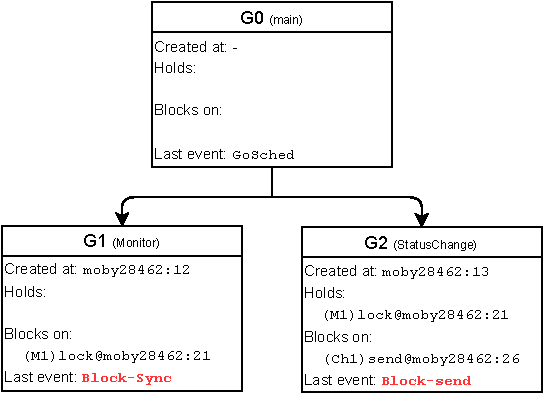
\includegraphics[width=0.9\linewidth]{figs/gtree.pdf}
%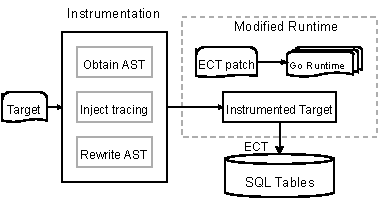
\includegraphics[]{figs/overview.png}
%\includegraphics[]{figs/overv}
\label{fig:gtree}
\caption{Goroutine tree of leaky execution of listing \ref{listing:moby28462}}
\end{figure}

Upon program termination, we construct a goroutine tree (figure \ref{fig:gtree}) of application goroutines by replaying through the execution ECT.
%
In addition to the parent/children relation of goroutines, nodes of the goroutine tree contains information about the goroutine creation site, the resources that it holds at each execution point and the final executed event right before program termination.
%
If tracing is enabled, every application goroutine invokes the tracer to capture $GoEnd$ before finishing its execution and exit (change status from \textit{grunnable} to \textit{gdead})\cite{goexit-line-of-code}.
%
Before the main function returns (\ie exits), it calls the scheduler (through \texttt{runtime.Gosched()} invocation which captures $GoSched$ event) to hand over the control to the root goroutine to finish up program execution.
%
Since we instrument the application to call \texttt{runtime.traceStop} to stop tracing when main returns, $GoSched$ would be the last event captured for the main goroutine if it returns succesfully.
%
We call an execution \textbf{successful}, if below conditions hold
\begin{description}
  \item (1) all goroutines spawned in the main goroutine has $GoEnd$ as their final event
  \item (2) the final event of the main goroutine is $GoSched$ with \texttt{runtime.traceStop} on top of its stack.
\end{description}


If either of above conditions does not satisfy after program execution, a \textbf{deadlock} happens because it shows that there are one or more goroutine that did not reach its final state. In other words:

if \texttt{finalEvent(}ECT.G$_{main}$\texttt{)} $\neq GoSched \Rightarrow Global Deadlock (GDL)$
else
  for ECT.G$_{appi}$ in application-level goroutines  :
    if \texttt{finalEvent(}ECT.G$_{main}$\texttt{)} $\neq GoSched \Rightarrow Partial Deadlock (PDL)$

    else:
    $Successful$

%
Other execution models such as figure \ref{fig:execVis} are also constructible when replaying the execution ECT.
%
\stcmt{I want to say that middlewares like DiffTrace and GOAT are helpful for human debuggers, because at the end of the day, nothing can be done fully automatically}
Human debuggers can use such models to review program execution and compare their expectations with actual behavior.
%
\stcmtside{future work}
Moreover, online or offline verifiers can take ECT as input and construct logical models to verify the program execution.
%


\begin{figure}[]
\centering

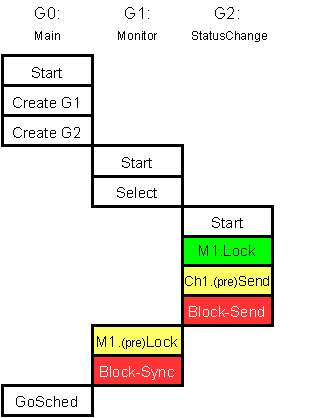
\includegraphics[width=0.6\linewidth]{figs/execVis.pdf}
\caption{Execution visualization of leaky interleaving in \ref{listing:moby28462} by replaying ECT}
\label{fig:execVis}
\end{figure}

\begin{figure}
\centering
  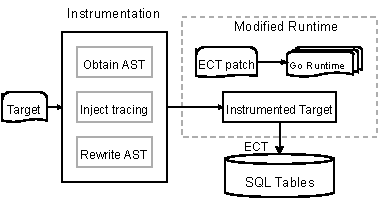
\includegraphics[width=.95\linewidth]{figs/overview.pdf}
  \caption{Framework Overview (NEED TO UPDATE)}
  \label{fig:overview}
\end{figure}

\subsection{Accelerating Bug Exposure}
\label{sec:critical}
As we have shown in figure \ref{fig:rare_bugs}, there are cases that the deadlock is hidden in the interleaving space.
%
It is proved that context-switches before synchronization/serialization operations in concurrent programs increases the probability of finding rare concurrent bugs \cite{burckhardt-depthBug-asplos10}.
%
For example, a rare context-switch right after the select statement in line \ref{bugListing:Monitor_select} causes the lock operation on mutex $m$ in line \ref{bugListing:Monitor_case_def_lock} of goroutine \texttt{Monitor} to \textit{block} goroutine \texttt{StatusChange} on locking $m$ in line \ref{bugListing:statChange_lock} and causing a deadlock.
%
Concurrency primitive usages are the \textit{critical points} in the program because their behavior directly impacts the blocking behavior of Go programs.
%
In \goat, we identify the usage of concurrency primitives as the critical points of the program before which a context-switch increases the probablity of manifesting a hidden bug that might not occur during conventional or stress testing.
%These critical points are interesting to study application correctness because 1)their behavior depends on the state of other goroutines at each execution step, 2) investigating their behavior and interaction with other goroutines is the key to debug the program behavior, 2) a contex-switch before their execution might change the operation behavior, and consequently the whole program behavior.
%
%
We define \textit{concurrency usage} (CU) as a triple of $<f,l,k>$ where $f$ is the file name, $l$ is the line number and $k$ is the kind of concurrency primitive used in the code location.
Kind $k\in$ \texttt{Channel} $\cup$ \texttt{Sync} $\cup$ \texttt{Go}:
\begin{itemize}
  \item \texttt{Channel} = \{\texttt{send}, \texttt{receive}, \texttt{close}\}
  \item \texttt{Sync} = \{\texttt{lock}, \texttt{unlock}, \texttt{wait}, \texttt{add}, \texttt{done}, \texttt{signal}, \texttt{broadcast}\}
  \item \texttt{Go} = \{\texttt{go}, \texttt{select}, \texttt{range}\}
\end{itemize}

The first column of table \ref{tab:moby_cov_table} shows the critical points extracted from program in listing \ref{listing:moby28462}.
%
We identify CU points by parsing the abstract syntax tree (AST) of the target source using Go AST package \cite{go-package-ast}.

CU points are passed to the instrumentation phase of \goat to inject scheduler perturbation handlers before these points.
%
%
%
% Through statically traversing the AST of any target package (e.g., files of the “main” package), goat gathers a set of line numbers where concurrency functions are used. These points (aka critical points) are the points where a context switch might drastically change the concurrency behavior of the program and trigger an undiscovered bug. Here are the AST nodes that represent a critical point:
% Go: ast.Node GoStmt   (example: go func() // spawning a new goroutine)
% Send: ast.Node SendStmt     (example: channel <- x)
% Recv: ast.Node UniExprStmt(op=”<-”) (example:  <- channel)
% Mutex, WaitGroup, CondVars: ast.Node CallExpr (example: xxx.Lock())
% Xxx.Lock()
% Xxx.Unlock()
% Xxx.Add()
% Xxx.Wait()
% Xxx.Signal()
% Xxx.Broadcast()
% Careful adjustment is required for Select and Range statements that have send/recv as their children in the AST.

\subsection{Instrumentation}
\label{sec:instrument}
\stcmt{below is the raw text that I wrote for instrumentation. I will complete it}
To equip the target application with concurrency tracing mechanism, we automatically inject three lines of code to the beginning of main or test function using AST package \cite{go-package-ast}:

\begin{itemize}
  \item \texttt{goat\_done := goat.Start()} initilizes \goat, enables tracing, and returns a channel as conduit between application space and \goat API.
  \item \texttt{go goat.Watch(goat\_done)} spawns a new goroutine as a watcher for liveness of the program (in case of global deadlocks or infinite loop). The watcher goroutine either receives from \texttt{goat\_done} and sends back an ack signal, or timeouts and stop tracing, and terminates.
  \item \texttt{defer goat.Stop(goat\_done)} sends a value to the watcher goroutine after main returns and signals that the program is finished. Then it waits to receive the signal from watcher, then stops tracing and terminates.
\end{itemize}

Additionally, to manipulate the native scheduler around CU points, we inject calls to \texttt{goat.handler()} before each statically discovered CU. \texttt{goat.handler()} randomly calls \texttt{runtime.GoSched()} to preempt the processing core from current goroutine and push the goroutine to the back of the global queue.



\begin{table}[]
\centering
\caption{Concurrency Usages and coverage requirements of program in listing\ref{listing:moby28462}}
\scalebox{0.9}{

\begin{tabular}{
>{\columncolor[HTML]{FFFFFF}}c
>{\columncolor[HTML]{FFFFFF}}l |
>{\columncolor[HTML]{FFFFFF}}l |
>{\columncolor[HTML]{FFFFFF}}c |
>{\columncolor[HTML]{FFFFFF}}c |
>{\columncolor[HTML]{FFFFFF}}c |}
\hline
\multicolumn{2}{|c|}{\cellcolor[HTML]{FFFFFF}CU of list. \ref{listing:moby28462.minipage}} & \multicolumn{1}{c|}{\cellcolor[HTML]{FFFFFF}} & \multicolumn{2}{c|}{\cellcolor[HTML]{FFFFFF}Covered by} & \cellcolor[HTML]{FFFFFF} \\ \cline{1-2} \cline{4-5}
\multicolumn{1}{|c|}{\cellcolor[HTML]{FFFFFF}Line} & \multicolumn{1}{c|}{\cellcolor[HTML]{FFFFFF}Kind} & \multicolumn{1}{c|}{\multirow{-2}{*}{\cellcolor[HTML]{FFFFFF}Coverage Requirements}} & run \#1 & run \#2 & \multirow{-2}{*}{\cellcolor[HTML]{FFFFFF}\begin{tabular}[c]{@{}c@{}}Overall\\      Covered\end{tabular}} \\ \hline
\multicolumn{1}{|c|}{\cellcolor[HTML]{FFFFFF}12} & go & covered & $\checkmark_{G0}$ & $\checkmark_{G0}$ & $\checkmark$ \\ \hline
\multicolumn{1}{|c|}{\cellcolor[HTML]{FFFFFF}13} & go & covered & $\checkmark_{G0}$ & $\checkmark_{G0}$ & $\checkmark$ \\ \hline
\multicolumn{1}{|c|}{\cellcolor[HTML]{FFFFFF}} & \cellcolor[HTML]{FFFFFF} & c-recv-blocked & $\checkmark_{G1}$ &  & $\checkmark$ \\ \cline{3-6}
\multicolumn{1}{|c|}{\multirow{-2}{*}{\cellcolor[HTML]{FFFFFF}17}} & \multirow{-2}{*}{\cellcolor[HTML]{FFFFFF}select} & c-recv-unblocking & $\checkmark_{G1}$ &  & $\checkmark$ \\ \hline
\multicolumn{1}{|c|}{\cellcolor[HTML]{FFFFFF}} & \cellcolor[HTML]{FFFFFF} & blocked &  & \cellcolor[HTML]{C0C0C0}$\checkmark_{G1}$ & $\checkmark$ \\ \cline{3-6}
\multicolumn{1}{|c|}{\multirow{-2}{*}{\cellcolor[HTML]{FFFFFF}21}} & \multirow{-2}{*}{\cellcolor[HTML]{FFFFFF}lock} & blocking & $\checkmark_{G1}$ &  & $\checkmark$ \\ \hline
\multicolumn{1}{|c|}{\cellcolor[HTML]{FFFFFF}} & \cellcolor[HTML]{FFFFFF} & unblocking & $\checkmark_{G1}$ &  & $\checkmark$ \\ \cline{3-6}
\multicolumn{1}{|c|}{\multirow{-2}{*}{\cellcolor[HTML]{FFFFFF}22}} & \multirow{-2}{*}{\cellcolor[HTML]{FFFFFF}unlock} & no\_op &  &  &  \\ \hline
\multicolumn{1}{|c|}{\cellcolor[HTML]{FFFFFF}} & \cellcolor[HTML]{FFFFFF} & blocked & $\checkmark_{G2}$ &  & $\checkmark$ \\ \cline{3-6}
\multicolumn{1}{|c|}{\multirow{-2}{*}{\cellcolor[HTML]{FFFFFF}25}} & \multirow{-2}{*}{\cellcolor[HTML]{FFFFFF}lock} & blocking &  & \cellcolor[HTML]{C0C0C0} \textbf{$\checkmark_{G2}$} & $\checkmark$ \\ \hline
\multicolumn{1}{|c|}{\cellcolor[HTML]{FFFFFF}} & \cellcolor[HTML]{FFFFFF} & blocked & $\checkmark_{G2}$ & $\checkmark_{G2}$ & $\checkmark$ \\ \cline{3-6}
\multicolumn{1}{|c|}{\cellcolor[HTML]{FFFFFF}} & \cellcolor[HTML]{FFFFFF} & unblocking &  &  &  \\ \cline{3-6}
\multicolumn{1}{|c|}{\multirow{-3}{*}{\cellcolor[HTML]{FFFFFF}26}} & \multirow{-3}{*}{\cellcolor[HTML]{FFFFFF}send} & no\_op &  &  &  \\ \hline
\multicolumn{1}{|c|}{\cellcolor[HTML]{FFFFFF}} & \cellcolor[HTML]{FFFFFF} & unblocking &  &  &  \\ \cline{3-6}
\multicolumn{1}{|c|}{\multirow{-2}{*}{\cellcolor[HTML]{FFFFFF}27}} & \multirow{-2}{*}{\cellcolor[HTML]{FFFFFF}unlock} & no\_op & $\checkmark_{G2}$ &  & $\checkmark$ \\ \hline
\multicolumn{1}{l}{\cellcolor[HTML]{FFFFFF}} &  & Coverage \% & 60\% & 33\% & 73\% \\ \cline{3-6}
\end{tabular}

}
\label{tab:moby_cov_table}
\end{table}


\subsection{Evaluation}

\stcmt{Experimental methodology - GoKer - Two main figures, one table I will add}
\begin{itemize}
  \item Figure \ref{fig:detection} : How \textbf{WELL} we detected bugs comparing to others
  \item Figure \ref{fig:runs} : How \textbf{SOON} we detected bugs comparing to others
\end{itemize}



\begin{figure}
\centering
  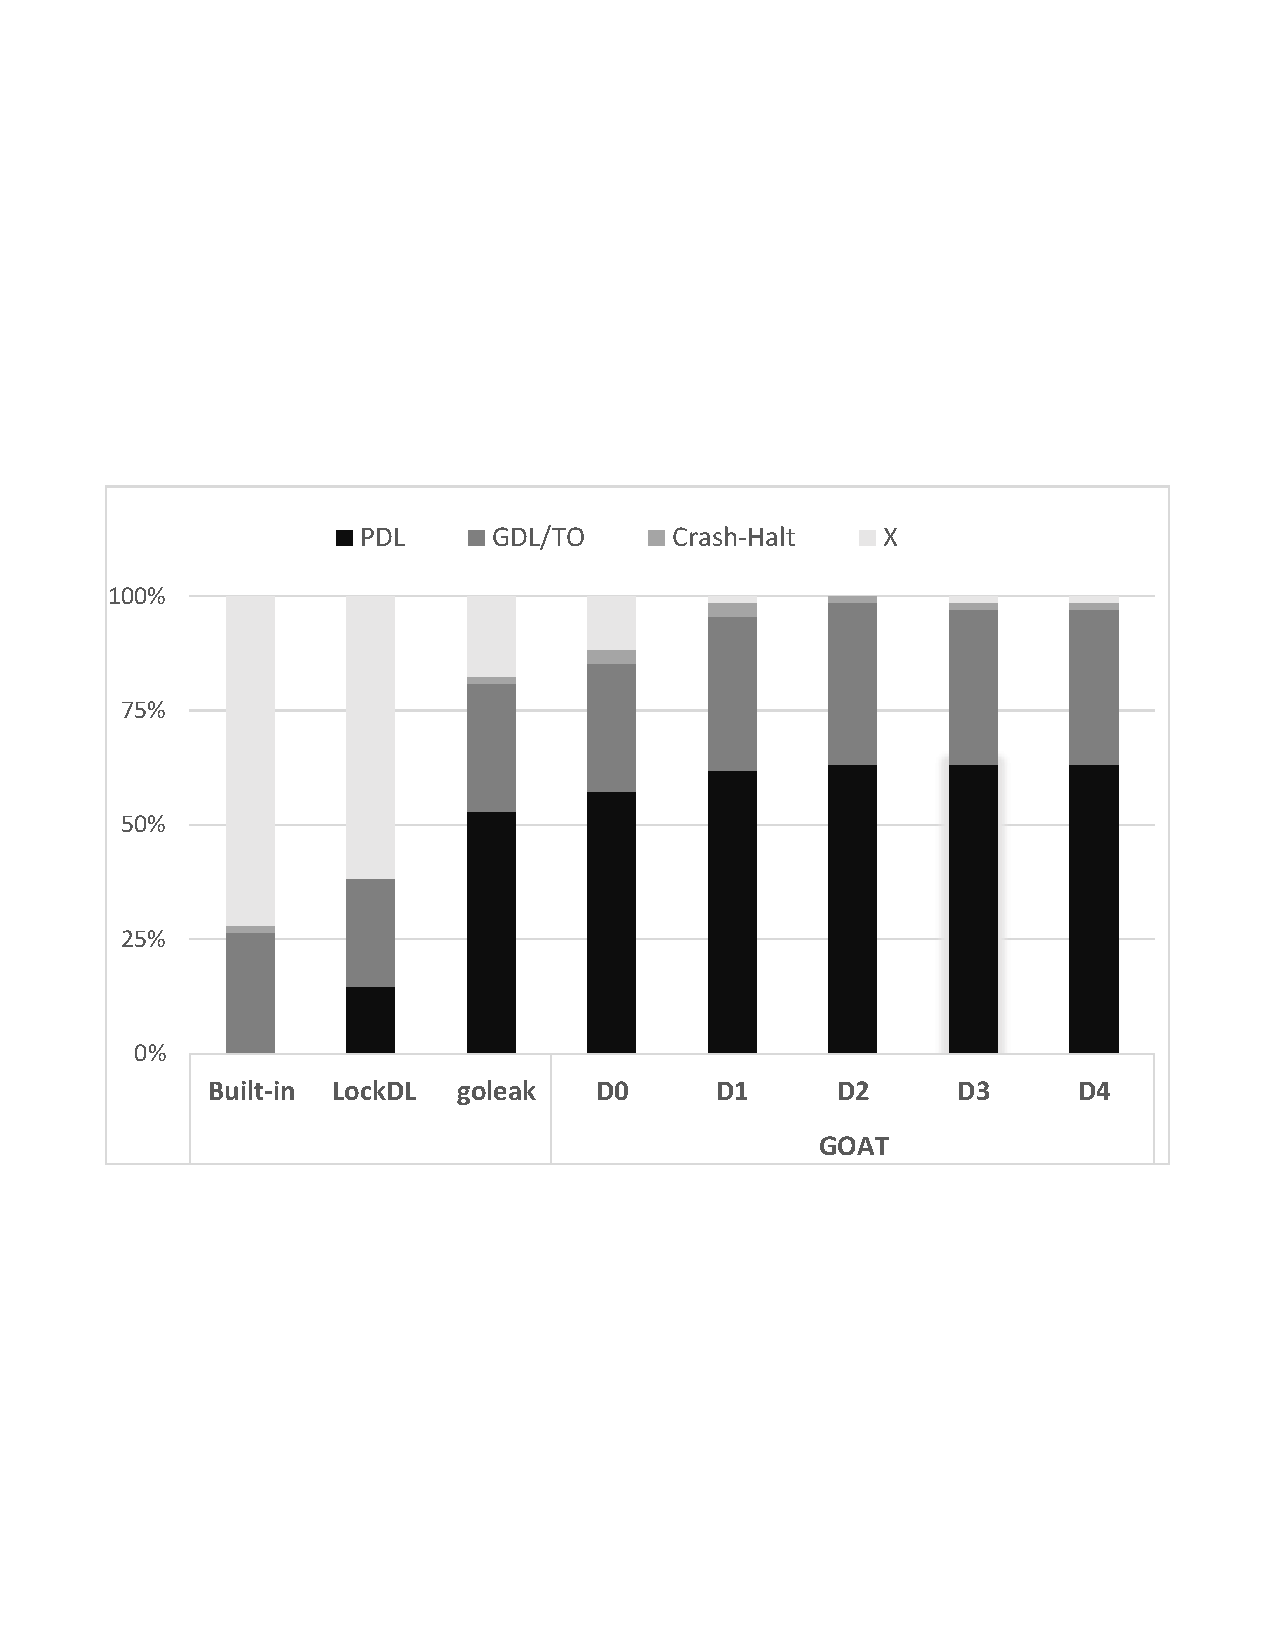
\includegraphics[width=.95\linewidth]{figs/P4_detections.pdf}
  \caption{Distribution of detected bugs by built-in deadlock detector (BUILTINDL), LockDL, GoLeak, and GOAT different d. (over 1000 runs). pdl: partial deadlock, gdl: global deadlock, crash/halt: causes the program to crash or halt on detection, x: nothing is detected }
  \label{fig:detection}
\end{figure}


\begin{figure}
\centering
  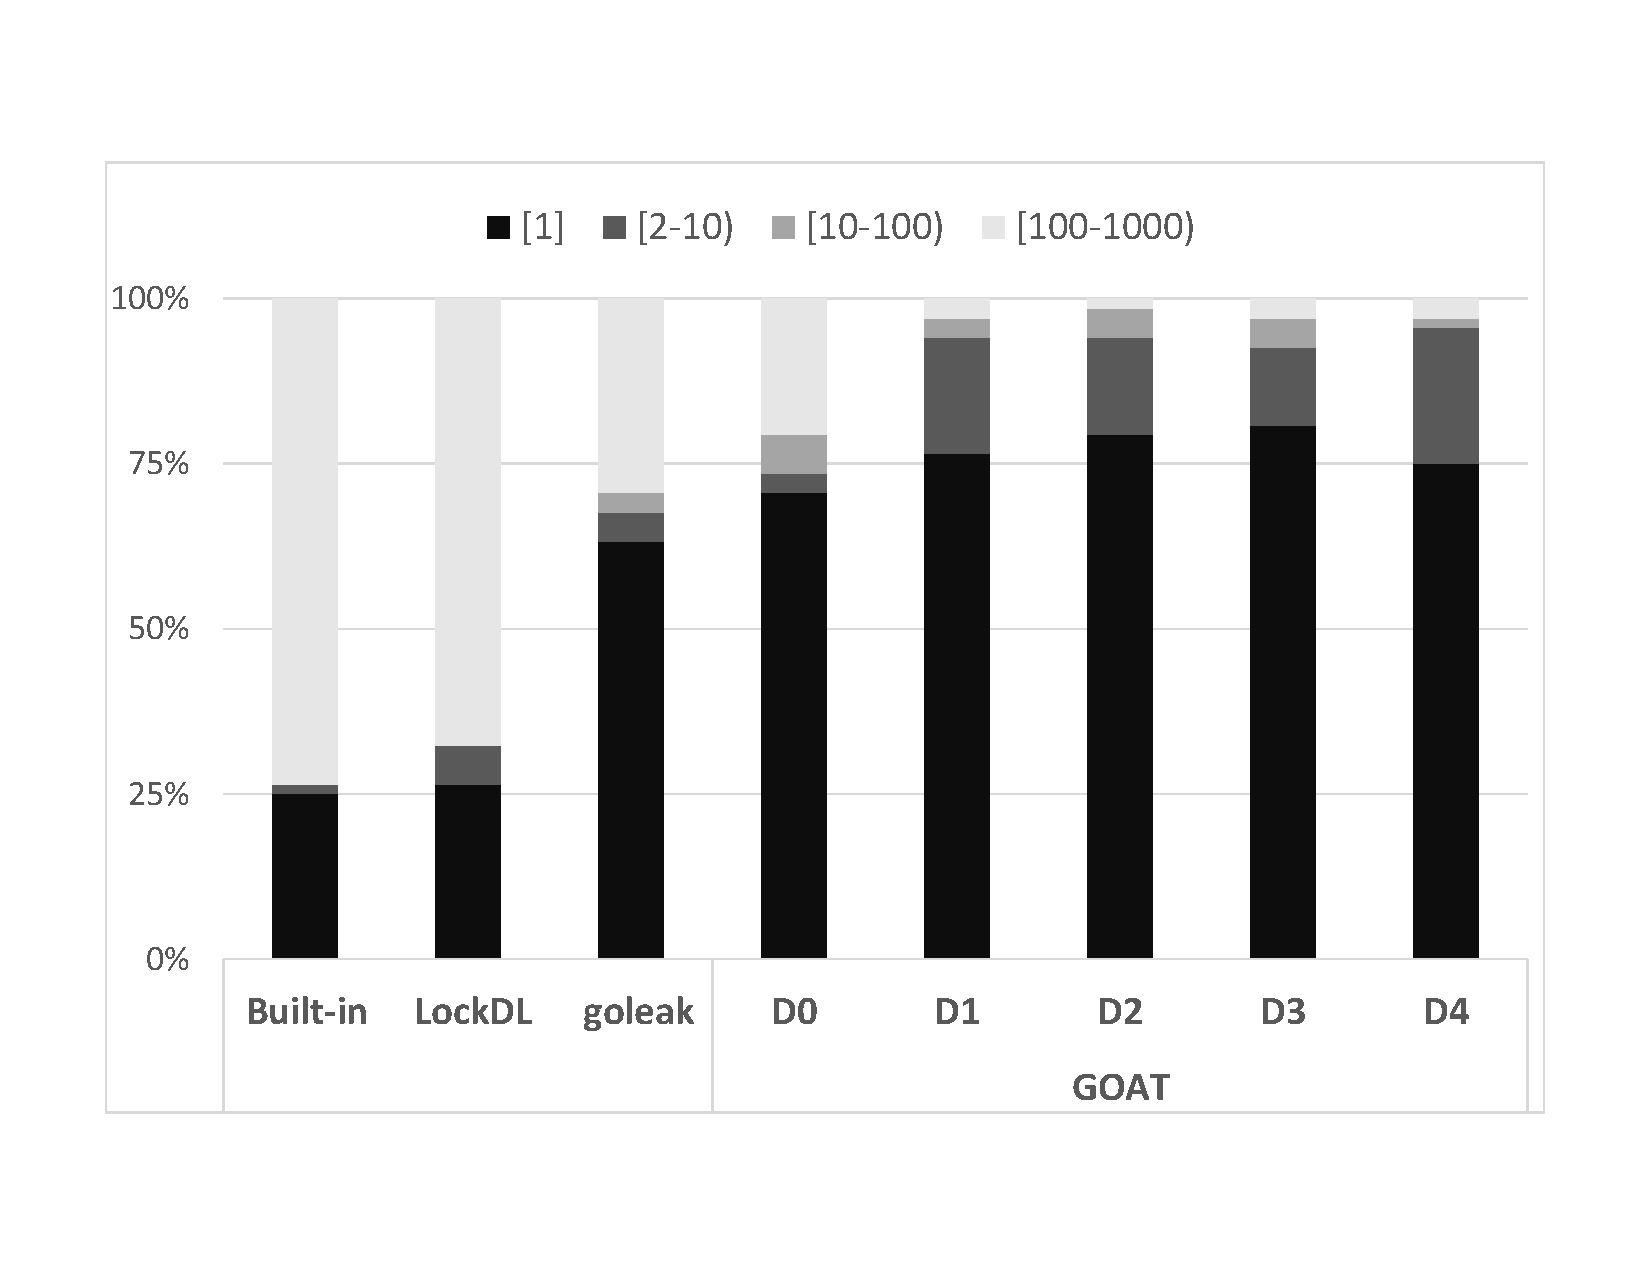
\includegraphics[width=.95\linewidth]{figs/P4_runs.pdf}
  \caption{Distribution of required number of iterations to detect the bug for each tool}
  \label{fig:runs}
\end{figure}
